% 来源：OEBPS/Text/Section0001_split_006.xhtml#sigil_toc_id_42

\BookChapter{30}
\section[第30章\q 超级富豪的秘密（你也可以用）]{第30章\\ 超级富豪的秘密（你也可以用）}

\begin{BookQuote}
那些超级富豪都把它看成圈里人的秘密：投资方式合法合规……只不过投资收益都不用交税。

\hfill ——《纽约时报》（2011年2月9日）
\end{BookQuote}

\subsection{寿险的新世界纪录}

2014年年初，吉尼斯世界纪录大全宣布，一个新的世界纪录诞生了，这并不是什么世界第一高人，而是一个大部分人没有注意到的世界纪录：

神秘的亿万富翁购买2.01亿美元的人寿保单，这打破了历史纪录。

为什么这个亿万富翁要买这么大的人寿保险？即使他提前离开人世，他有那么多钱，他的孩子也一样会过得很好。是不是媒体没有抓住重点？不管你信还是不信，那些超级富豪确实购买了天文数字般的人寿保险，但是买得最多的并不是那些亿万富豪，最大的买家是银行和大企业，从沃尔玛到富国银行，都大买人寿险。例如富国银行的资产负债表显示，其一级资本中存到人寿保险上的现金价值为187亿美元（截至2014年5月27日）。要知道，一级资本可是一家银行的财务实力的核心衡量指标！与媒体所说的相反，大公司、大银行和超级富豪大买人寿保险，并不是想从任何人的死亡中获利。他们真正想要的是，找个地方来存放他们的现金。作为一种美国税务局批准的工具，那里允许他们的投资增值免于纳税。这听起来太好了，简直不像是真的。事实上，这在税收待遇上非常像罗斯个人退休金账户。你赚到的钱（收入），交了所得税，但是一旦你把这些纳过税的资金放到一个特殊类型的人寿保险里，美国税务局就同意，这笔投资以后的增值就不用再交所得税了，如果结构安排正确（后面详述），当你从保单里把钱拿出来的时候，你也不用交税。所以尽管这是人寿保险，却不是你死了才能赚钱，而实际上它是精心设计的，在你活着的时候用来从中获利的。

这种特殊的人寿保单，对于亿万富翁和世界上最大的公司来说，再好不过了；对于我们这些普通人来说，也可能是再好不过了。让我们仔细研究一下，看看如何利用这种强大有力的避税工具，来加快我们的财富积累速度，提早实现财务自由。

\subsection{富人的免税账户}

后面要讲的策略属于私募人寿保险，《纽约时报》称之为富人的秘密，这个说法非常贴切。这个工具就是我认识的两位超级富豪推荐给我的，但是你并非一定要是超级富豪才能利用这种工具的优势。很多高收入人士，包括医生、律师、小企业主，也会从后面我们要讲的人寿保险投资知识中发现巨大的应用价值，但是那些只有几千美元闲钱的普通人将会学到如何创造一个类似版本的投资结构，给你提供同样的好处。所有人都可以得到以下令人震惊的好处：

\begin{itemize}
\item 存入资金数量没有限制（没有最高收入限制）
\item 投资增值不用交税
\item 提现不用交税（前提是结构安排正确）
\item 留给你的继承人的所有钱都不用交税
\end{itemize}

我们不要觉得这个工具是一种很酷的策略，就一带而过。这本质上是把你的一部分或者全部养老金从税收体制中全部挪走了！这样一安排，你以后的投资增值再也不用交税了，你以后的投资取现再也不用交税了。这正是媒体为什么称私募人寿保险是富人的“免税投资账户”。好好思考一下登在《华尔街日报》上的那篇文章《如何创造一份养老金》中的一段话：

最主要的吸引力：因为你持有的投资外面包装了一层人寿保险，所以保险里面实现的投资收益可以免缴收入所得税，直到你死后才用纳税。另外，保险持有人可以拿到他们的钱，就在他们活着的时候，可以提前取现，也可以用保险贷款，完全免税，具体数额取决于保险的产品结构设计……这种人寿保险销售大幅增长，一个很大的原因是，最近几年，美国国税局发布了一系列的规章制度，里面说得很清楚，私人订制的人寿保险和年金，哪些允许免税，哪些不允许免税。相应地，这消除了保险公司和投资者之间的不确定性。

把税收从投资等式中拿出来之后，你的财富积累速度会大大加快，让你能比计划提前好多年到达你的财富关键规模目标和财务独立所需的财富目标。你再也不用担心，你赚的钱究竟有多少是你可以花的，因为税务局的人会先把你的苹果咬一大口，事实上，想知道你未来真正需要多少钱才够，面临的一个最大的困难就是，你不知道你未来要交税的税率会是多少。记住，税收很容易就会提高，突然之间，所得税提高了，自然你的可消费收入就减少了。如果你做投资理财规划的时候，用的是50\%的所得税税率，但是到了你预计的将来，对富人征收的税率提高到了70\%，或者现在你的所得税率是30\%，到你预计的未来，你这样的收入等级的所得税税率提高到了50\%，那么原来你做的投资理财规划的收益，在税率提高后，你实际拿到手的钱就达不到你财务自由的目标了。

我们来看一个案例，你如何运用这种工具，只用原来计划的一半时间实现财务安全或者财务独立，抑或是你保持同样长的投资期限，最后你真正到手可以随意消费的资金数量增加1倍？

如果你是一个高收入人士，就像医生、牙医、律师、小企业主，你很幸运，每年税前收入能达到25万美元。收入高，所得税也高，意味着交过所得税之后，假定联邦所得税和州所得税的合计税率为50\%，你能拿到手的税后净收入只剩下12.5万美元。你一年正好需要12.5万美元，才够维持你现在的生活方式，挣的越多，花的越多。这12.5万美元就是你每年的全部可消费收入。传统的投资理财规划是，你需要积累的财富是你现有年收入的20倍，也就是说，你的关键规模必须达到500万美元，才能产生25万美元的税前收入（假定提现比例为5\%）。如果国家不要求你交税，那么你需要的实际年收入是12.5万美元。你实际上只需要积累12.5万美元的20倍，或者说，在现在这种结构安排下，总的关键财富规模只需要250万美元就够了。这意味着你到达你的财富目标的速度快了50\%，或者说，你用同样的时间到达你原定的财富规模目标，这让你得到的可消费收入增加了1倍。

如果你收入不高，一年只能赚到5万美元，你会说：“那又怎样？这种人寿保险难道不是只对那些有钱人有好处吗？”别着急，你先听我讲富人怎么利用这种人寿保险来避税的。接下来，我会讲普通收入阶层也能利用这种人寿保险来避税，加快财富积累，让你实现财务目标的时间加快30\%\textasciitilde{}50\%，而且所有这些避税的产品都能得到美国税务局的支持，就像支持401(k)计划或者罗斯计划一样。

\subsection{人寿保险贵吗？}

我的律师第一次跟我谈到私募人寿保险时，我一听就觉得非常反感。跟大多数人一样，过去碰到太多人向我推销昂贵的“零售”人寿保险了，我再也不想让那些卖保险的家伙欺骗我了。

我的这位律师接着解释道：“托尼，这并不是那种你平时经常见到的零售人寿保险。那种见人就推销人寿保险的推销员，发型做得很帅，开着一辆金色的劳斯莱斯，但是你从他那里根本买不到这种人寿保险。这是一种机构定价的保单，没有佣金，没有退保手续费，也没有你遇到的那些零售代理人碰到你时讲的那一大堆废话。你可以把这种人寿保险想象成只是在外面包了一层‘保险的皮’，其实你买的是一个用来放置你投资的地方，你放到这里的所有投资都可以合法地避税，只要在这层保险的包装里面就行。这种人寿保险里的资金可以投资到各种各样的基金，你的投资增值不用交税，如果我们操作正确的话，你从保险里提出来的现金也不用交税。”

\subsection{免税复利增长}

复利增长的时间长了，这种私募人寿保险带来的好处会大得惊人。我们来看一个案例，两个保单投资相同，只不过一个包装在这种私募人寿保险里面，不用交税，另外一个就是标准的做法，每年要交税。

假设一个健康的男性，现在45周岁，每年存入25万美元，连存4年，累计存入100万美元，如果他能得到10\%的投资收益率，而且必须年年交税，那么过了40年，他的账户余额总额会是700万美元。还不错，是吧？但是如果他把投资包装进一个私募人寿保险，相对而言他只是支付一笔很小的费用作为保单的费用，他的最终账户余额（保单现金价值）超过3000万美元！同样的投资策略，他实际拿到自己手里的钱高了4倍（400\%），这样他和他的家人能够花的钱就多了4倍，关键在于他能运用税法来合理避税。（请记住，对投资管理有非常严格的法律法规约束，必须由一个第三方投资专业人士来投资操作，而不能由保单持有人自己操作。）

顺便说一下同样强大有力的好处，甚至也可以被用在规模更小的投资上，它就是不用交税的复利增长！但是接下来我想知道，我若想取出保单里的钱，该怎么办。

\begin{figure}[htbp]
\centering
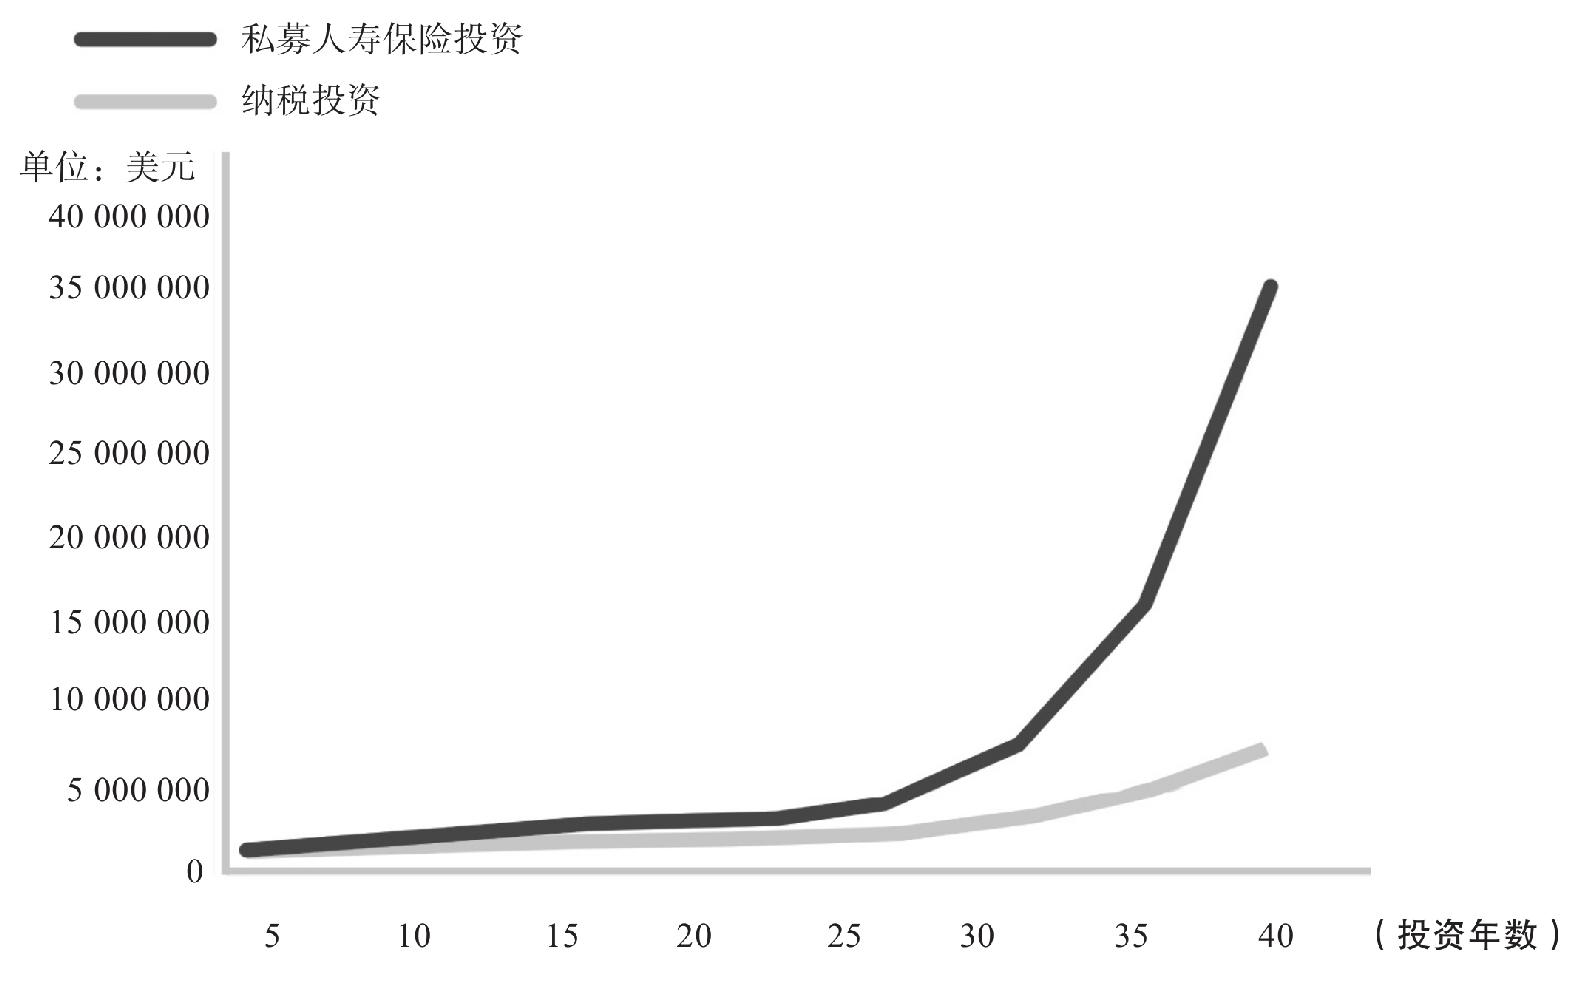
\includegraphics[width=0.92\linewidth,keepaspectratio]{image/30-1.jpg}
\caption{}\label{fig:30-1}
\end{figure}

\subsection{把保险里的钱取出来}

私募人寿保险的威力在于，你不需要担心将来的税率是多少，在你一生投资的过程中，只要是在这个保险里的投资产生的收益，你就不用纳税，钱全都是你自己的。但是如果你需要现金呢？那么就像政府批准享受税收递延优惠的其他投资工具一样，提现就必须交税，但是你有权力从你的保险里借钱，换句话说，你可以打电话给保险公司得到一笔现金，相当于你的保险现金价值，但是从法律上讲它是一笔贷款，这笔贷款是不用交税的。到了你选定的还款日期，你可以归还贷款，你如果去世了，就用人寿保险的分红来归还贷款。这是合法的贷款，它确实能让你拿到现金。还有没有别的巨大好处？人寿保险受益人得到的死亡赔付款是免税的，所以你的孩子收到这些赔付款的时候不用交税。

\subsection{你有资格吗？}

要购买私募人寿保险，和购买私募基金一样，你必须是他们所说的合格投资者\footnote{\label{fn:pdf-30-1}要有资格购买私募人寿保险，你必须成为一个合格投资者。这意味着你的财富净值至少要有100万美元（不包括你的主要住所的价值在内），或者你最近两年每年至少要有20万美元的收入（或者你和你的配偶合计每年收入为30万美元）。}，而且一般要求每年最低存入年金25万美元，至少要连存4年。不过，还有一个版本的私募人寿保险，现在哪怕你只有几千美元也可以投资。美国教师退休基金会是1918年由当时很有远见的安德鲁·卡内基设立的，目标是服务教师，而不是为了给公司或者给股东带来利润。现在美国退休教师基金会也给公众提供金融服务，但是这个基金会独一无二的非营利结构允许其提供人寿保险产品，既不收销售手续费，也不收退保手续费。在这样的保险里面的资金投资选择包括低成本的指数基金，这些基金完全符合本书里很多投资专家给我们的投资建议。税收上的好处和我们前面了解到的私募人寿保险没有什么不同。记住，作为一个无手续费也无佣金的保险产品，根本没有保险代理人会敲你们家的门来推销这种产品，所以你需要访问基金会的网站，自己动手购买或者找一个受托人理财顾问来帮助指导你买一份保险。

作为受托人，你的代表不能收取佣金。如果他在这方面很有技巧，而且完全了解如何设置这样一个有税收效率的策略，他就能为你提供优质的服务。基于你现在的税率，这种人寿保险能帮助你更早地实现你的财务目标，时间会提前30\%\textasciitilde{}50\%，没有任何附加的风险。当然，如果你是堡垒投资理财公司的客户，我们会有一个团队来为你安排所有这些细节。

\subsection{亿万富翁战术手册}

我们一起走了这么长的投资旅程！我们和瑞·达利欧一起征服了丛林，学到了如何设计一个投资组合，安度所有经济季节，为你持续提供平稳的收入接近75年之久。我们学会了如何创造一个有保障的终身收入计划，能够获得上行收益，而且没有下行风险，使用的工具就是收入保险。在这个部分的最后，我们了解了一个非常少见的无佣金人寿保险，它能给我们带来等同于罗斯账户的免税好处，却没有收入和缴费金额的限制。现在是时候得到机会——礼物了，让你能够坐下来直接向一些投资世界最优秀的大师学习，倾听他们的心声，了解是什么把他们塑造成现在这个样子的。他们会告诉自己的孩子什么东西，来教育孩子成为一个成功的投资者？现在让我们翻到下一部分，跟大师面对面。

\subsection{生前信托}

还有一点要讲一下，它很简短，但是很重要。那些富豪都费尽心机做好投资理财规划来保护他们的家庭。有些特别简单的事情，你一做就能保护好你的家庭，其中之一就是建立一个可撤销的生前信托。用生前信托来持有你的核心资产，包括你的房子、证券交易账户和你的交易账户等，最大的好处就是，一旦你去世了，这些财产可以避免法庭认证。法庭认证要走一套程序，成本高且时间长，让法庭盘点你的财产（每样东西都要做成公开记录）。但是和遗嘱不一样，生前信托也可以在你活着的时候保护你和你的家人。如果你生病了或者没有行为能力了，你可以在生前信托里面加入一个无行为能力条款，允许某人做继任受托人，处理你的账单和其他事务。但是不要听信那些专家说一个生存信托要花费好几千美元，你可以在网上得到一个免费的模板文件。香奈儿·雷诺兹就创办了这样一个非营利网站，那是在她丈夫骑自行车时因交通事故死亡之后，她想确保没有人再次经历这种毫无准备的痛苦经历。

我在这时特意附上生前信托这个提醒，是因为即使本书的目的并不是要成为一个遗产规划工具，我们也都要承担一个重要的责任，就是不管我们积累的财富是什么样的，不管这些财富是大还是小，都要确保我们的家人能从中受益，不会陷在一个法律程序里，让它吸干我们要留给继承人的礼物。如果你已经积累了一些财富，请寻找高质量的帮助，帮你做好遗产规划。不要再等了，马上设立一个生前信托。每个人都需要设立一个生前信托。
